\documentclass[../main.tex]{subfiles}

\chapter{Spoof simulation test}
When a GNSS receiver is spoofed, its solved position or time (or both) might change. The result depends on the technique used to spoof. By moving a GNSS receiver, one can simulate a spoofing attack since the location most certainly will change. It might also affect the time solved (but why? Figure this out). We also covered the antennas with aluminium foil to simulate a loss of signal.

\section{Data acquisition}\label{data_aquisition}
In order to create an accurate clock-model of the CSAC, it was necessary to log data from it while it was running in a disciplined mode. In the disciplined mode, the CSAC will correct it's frequency based on either a 1 PPS (Pulse per second) signal or a 10 MHz signal as discussed earlier (\ref{csac_com}) A similar approach was used in order to collect GPS data. Data from two u-blox NEO-M8T was gathered over the same time period as the data gathered from the CSAC. By gathering the data over the same period, it was possible to detect any correlation between the time solved by the GPS receivers and any frequency adjustments done by the CSAC. It also provided valuable data that could be used to tune the spoofing detection algorithms in the CSAC SMACC. The data gathering was done by simple Python scripts (\ref{CL} and \ref{GL}) running on a computer connected to the receivers and the CSAC (\ref{CLS})

\subsection{Setup}
\begin{figure}
\centering
  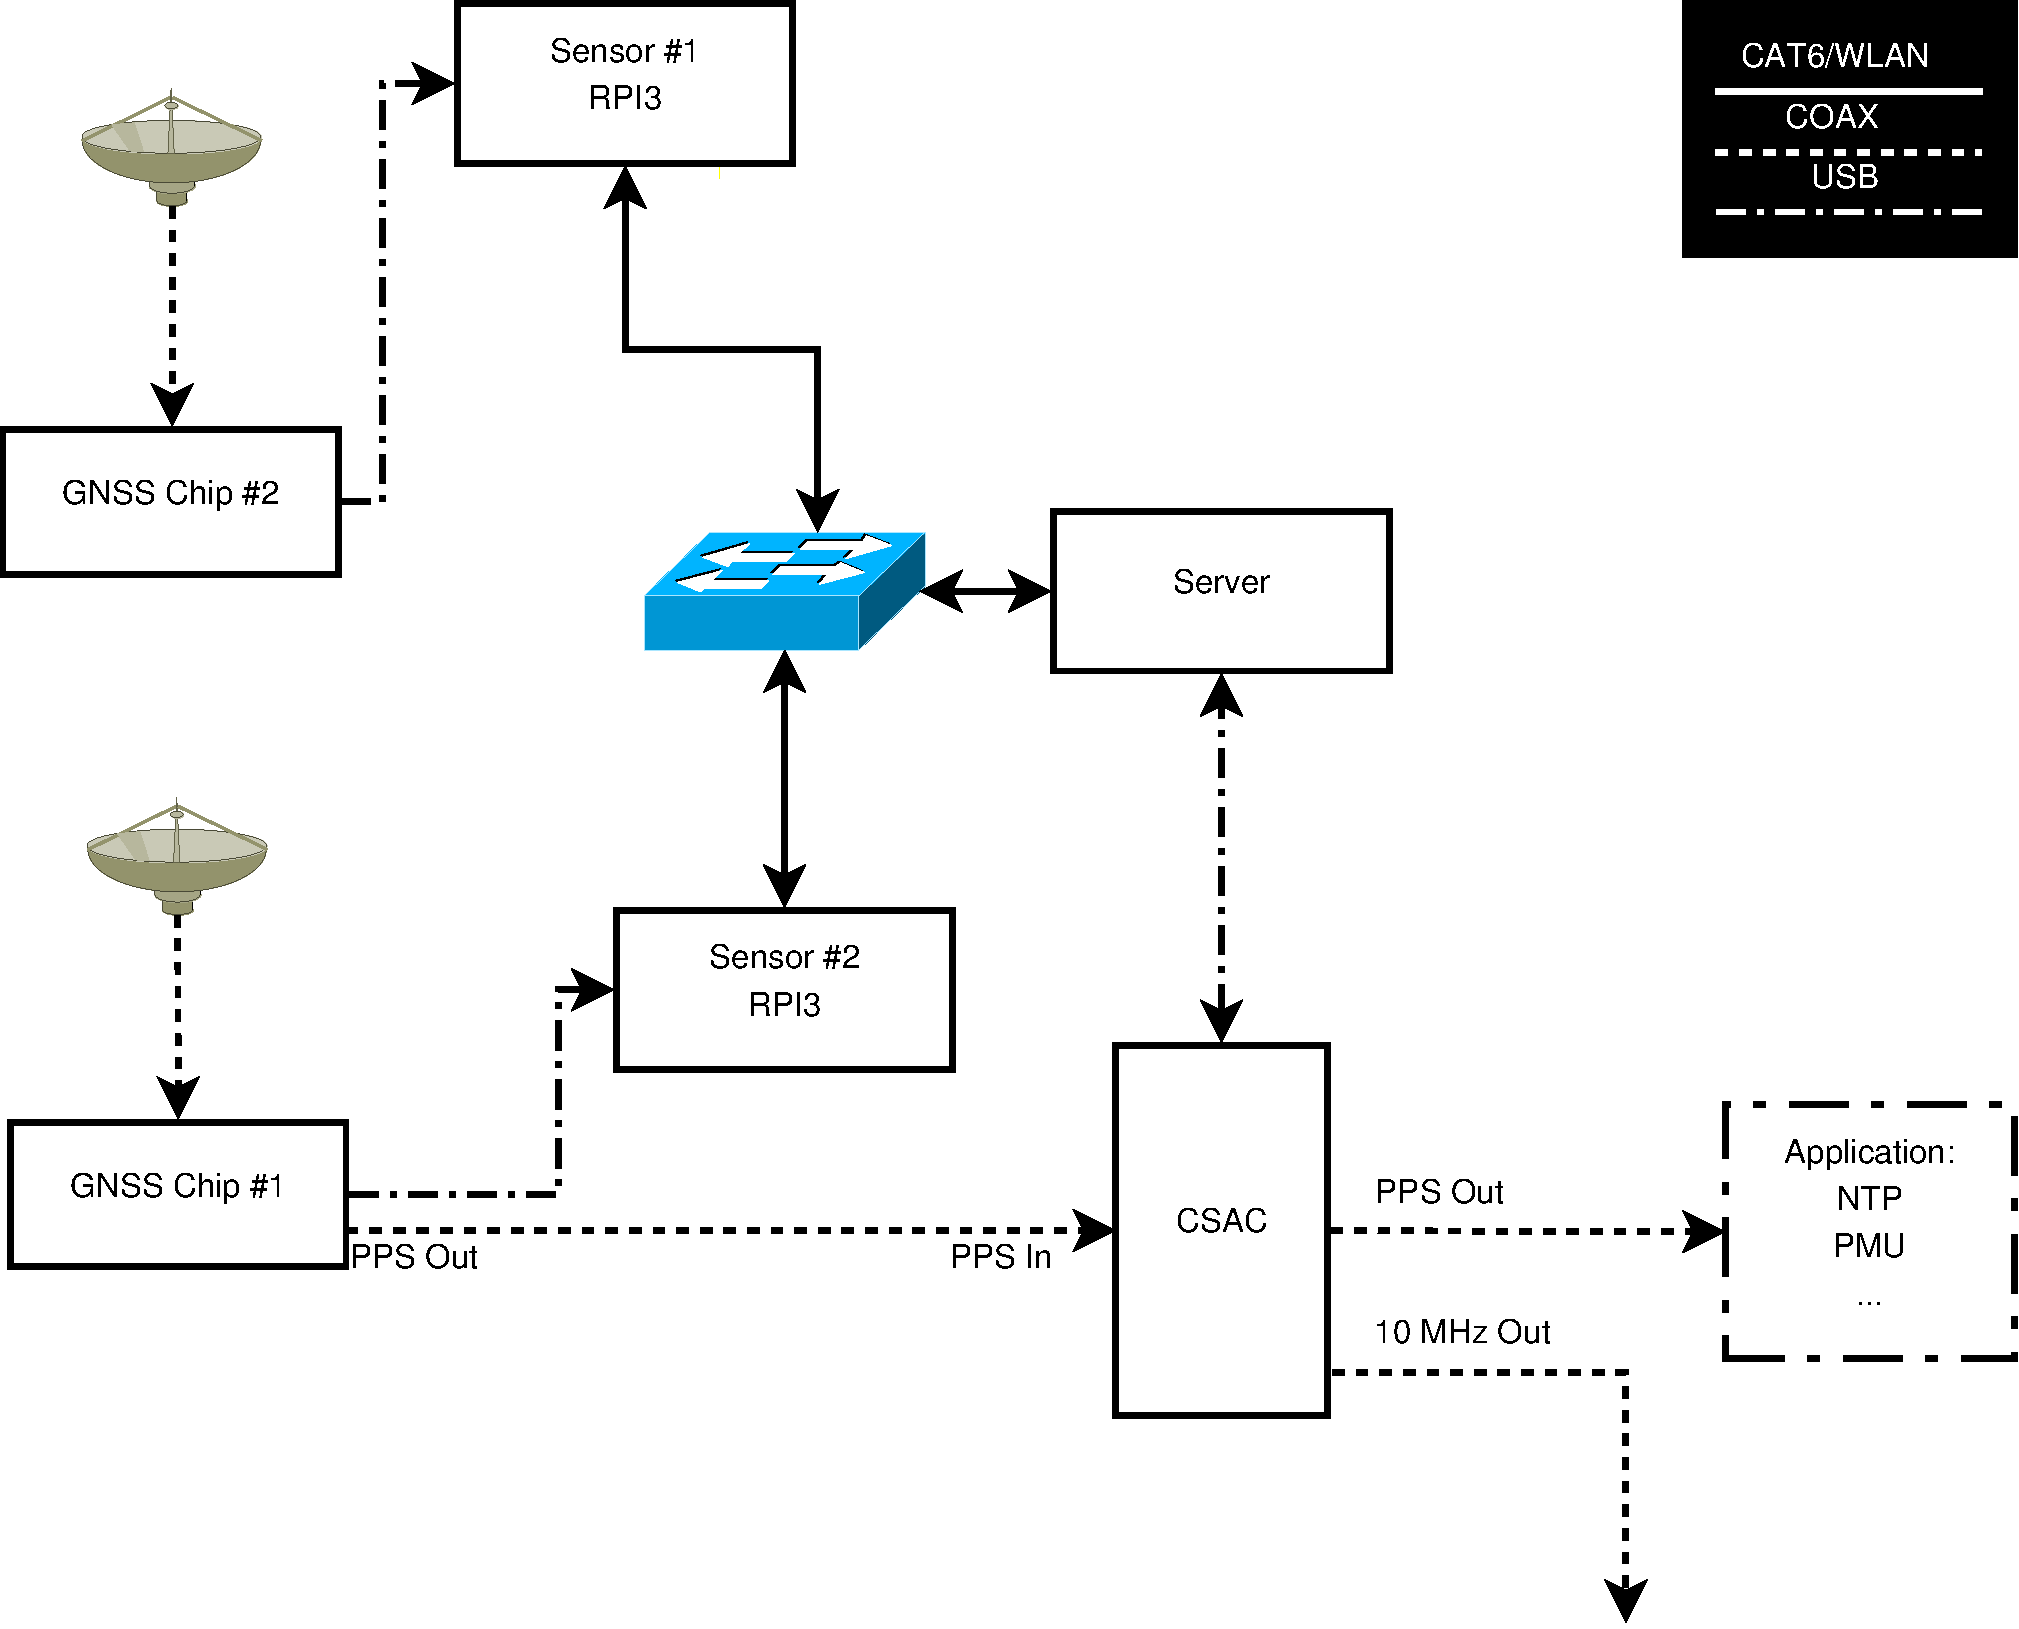
\includegraphics[scale=0.31]{server_layout.pdf}
   \caption[CSAC SMACC implementation block diagram]{A block diagram showing the tested implementation.}
   \label{ibd}
\end{figure}
Figure \ref{ibd} shows how the Server, Sensors and CSAC where physically set up. In order to assure good GNSS satellite geometry, the antennas where placed at the roof of Justervesenets main office at Kjeller. Antenna 1 was placed at a railing about a 1 meter above the ground, antenna 2 was placed at ground level. Antenna 1 was connected to GNSS receiver 1 which in turn was connected to Sensor 1. It's the same deal with antenna 2 which was connected to GNSS receiver 2 which in turn was connected to Sensor 2. The distance between the two antennas was about 35 meters. The Sensors and the Server where connected to LAN through a Gigabit ethernet switch. The Server was configured to log telemetry received from the CSAC and the Clients where configured to log all NMEA data received from the GNSS receivers. The GNSS receiver connected to antenna South is used to supply the CSAC with a 1 PPS signal. Because the CSAC model needs live data over time to mature, the system was started Friday 7. October and the test was performed Monday 10. October.

\begin{figure}
\centering
  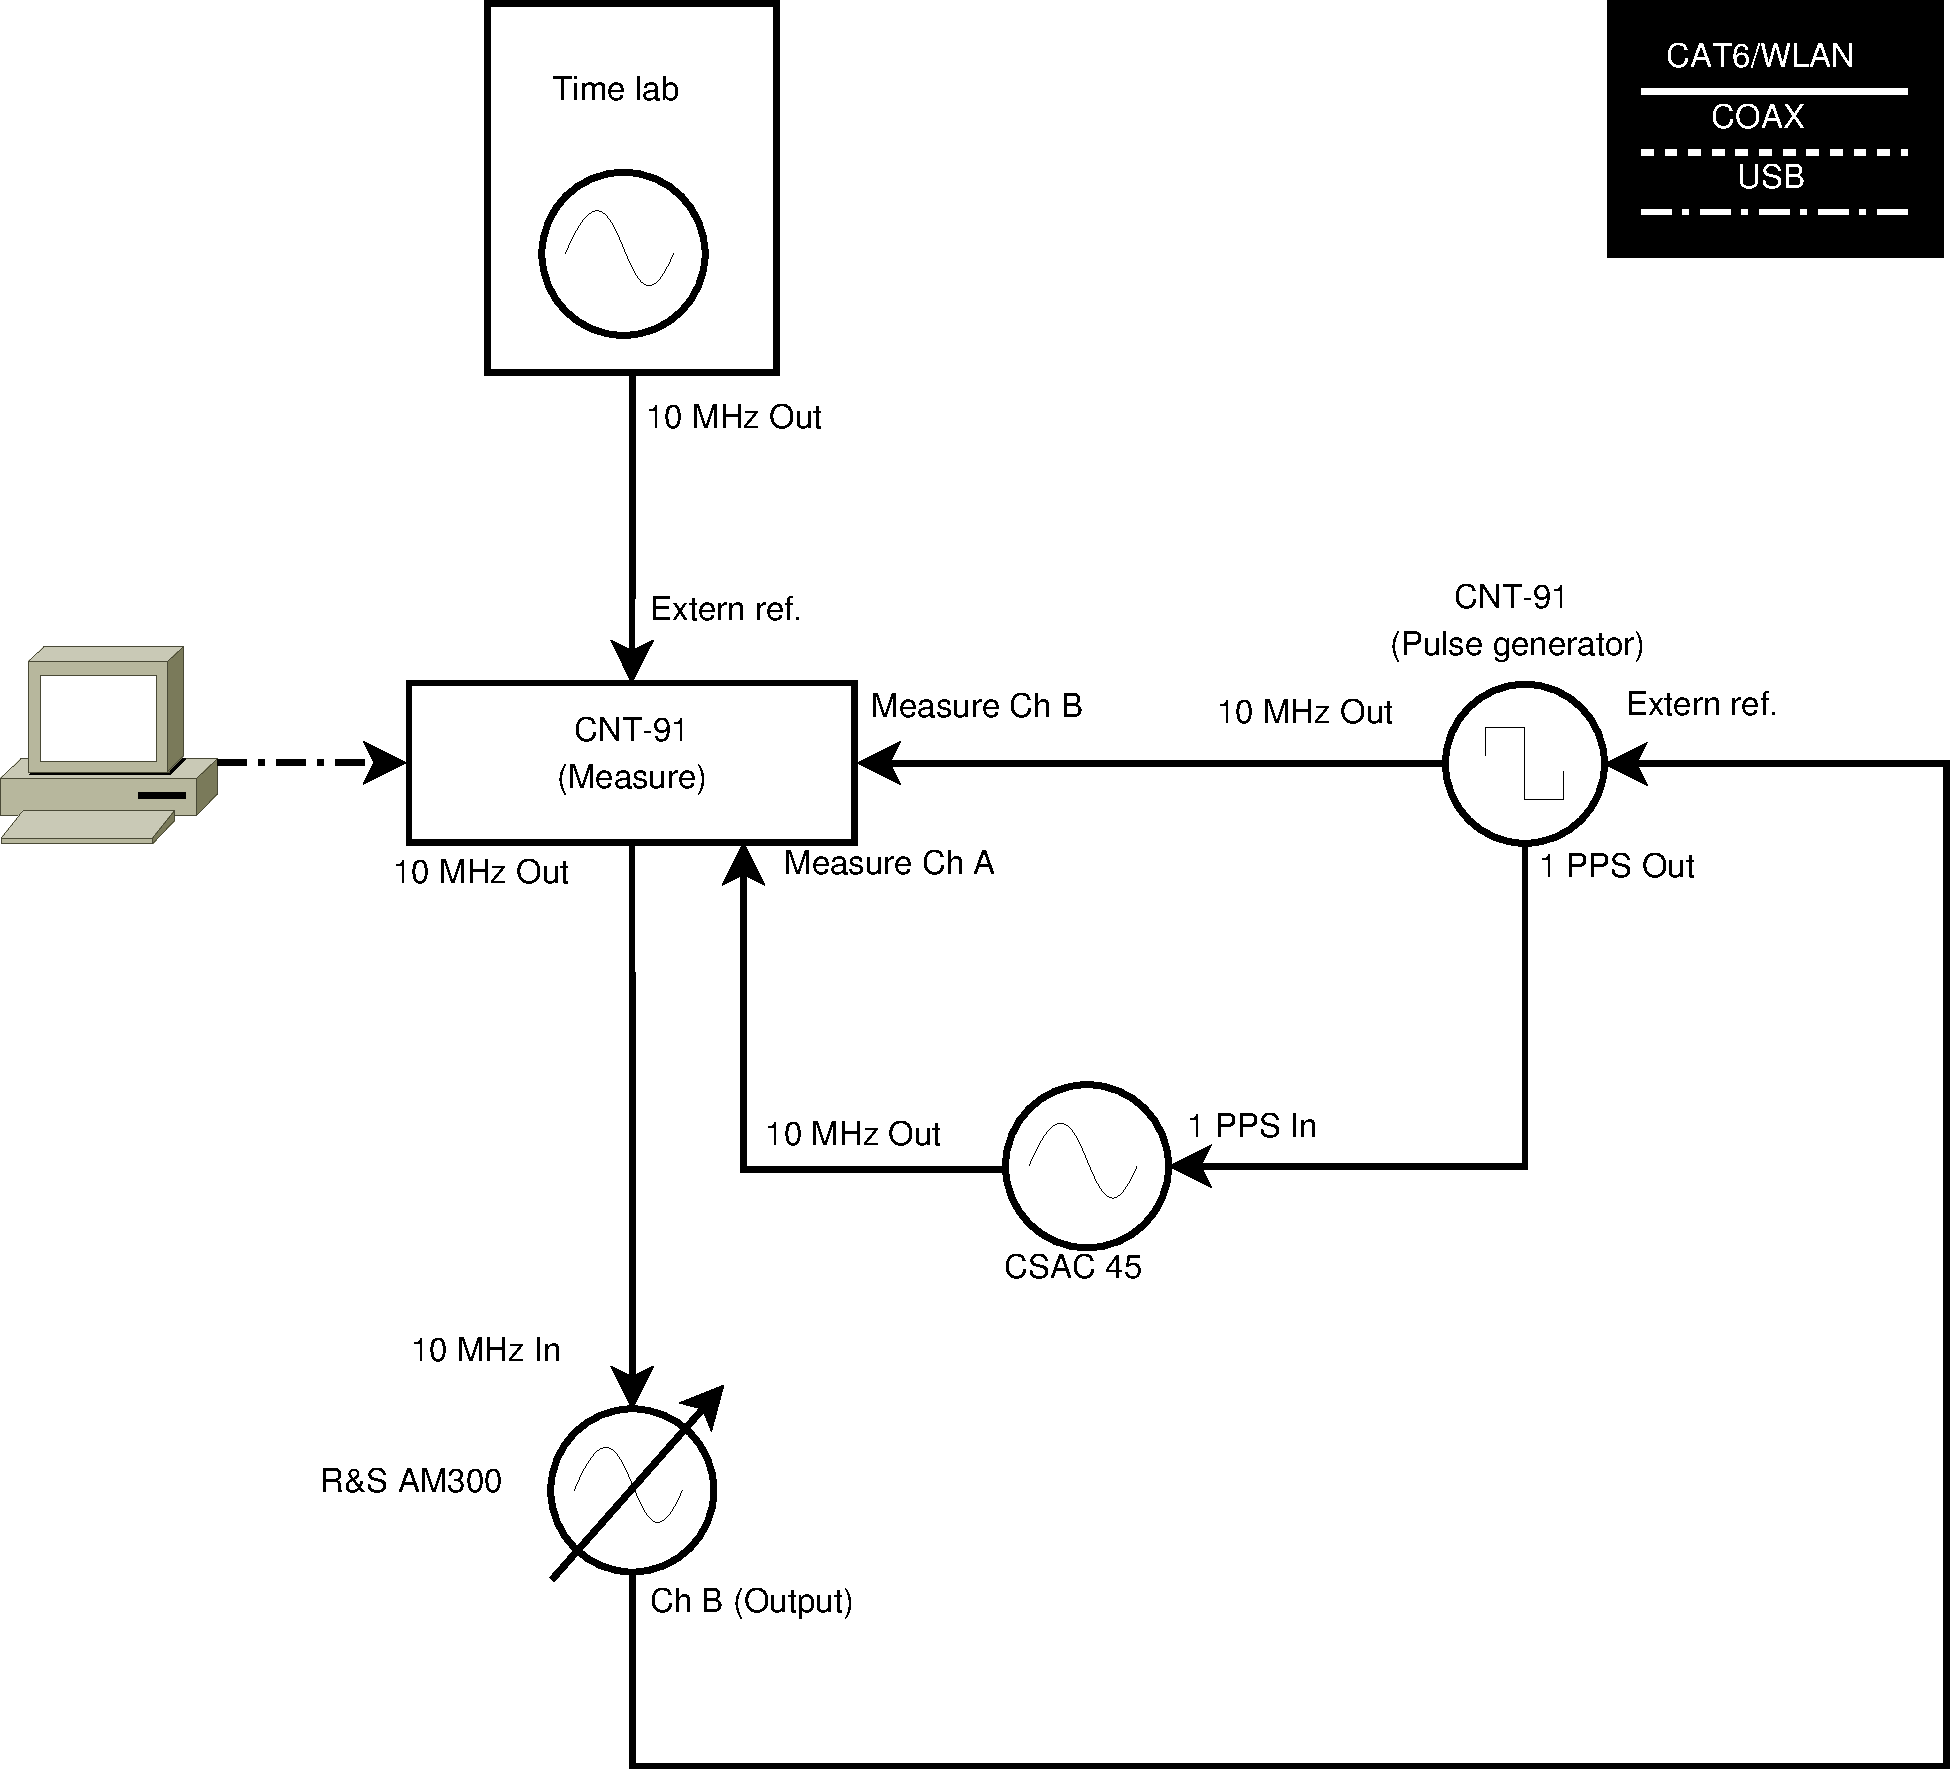
\includegraphics[scale=0.31]{measure_setup.pdf}
   \caption[Measurement setup]{Block diagram showing the setup of the measurement equipment}
   \label{msd}
\end{figure}

\subsection{Goal of test}
The goal with this test was to use the CSAC SMACC to detect a simulated spoofing attack. By moving the antennas, the KRL filter(\ref{kvsrlf}) should be triggered as the solved longitude, altitude, latitude and speed should change. The CM might also trigger. The result would be observable by analyzing the log files produced by the Server and Clients and the data collected by the measuring setup.

\subsection{Description}\label{description}
The following is a step by step description of how the test was conducted. The time in the brackets was obtained from a wristwatch. It is written in the normal format as well as number of seconds after 10:48. This is because the data used to draw the graphs, started at 10:48 but uses seconds in the X axis. Comparison is therefore easier. It is important to note that neither the resolution or accuracy was of any notable concern when writing down the time. The time was mainly noted to make it easier to find any correlation between the steps taken and patterns found in the log files. 

\begin{itemize}
  \item\relax 10:58 - 600: Moved antenna 1 approximately 15 meters to the south.
  \item\relax 11:03 - 900: Moved antenna 1 back to original location.
  \item\relax 11:07 - 1140: Moved antenna 2 approximately 15 meters to the north.
  \item\relax 11:12 - 1440: Moved antenna 2 back to original location.
  \item\relax 11:14 - 1560: Waved antenna 1 around horizontally in a half circle motion at an increasing tempo.
  \item\relax 11:18 - 1800: Waved antenna 2 around horizontally in a half circle motion at an increasing tempo.
  \item\relax 11:20 - 1920: Covered antenna 1 with aluminium foil.
  \item\relax 11:25 - 2220: Covered antenna 2 with aluminium foil.
  \item\relax 11:28 - 2400: Removed foil from antenna 1.
  \item\relax 11:33 - 2700: Removed foil from antenna 2.
\end{itemize}
\newpage

\begin{wrapfigure}{r}{0.40\textwidth}
  \centering
  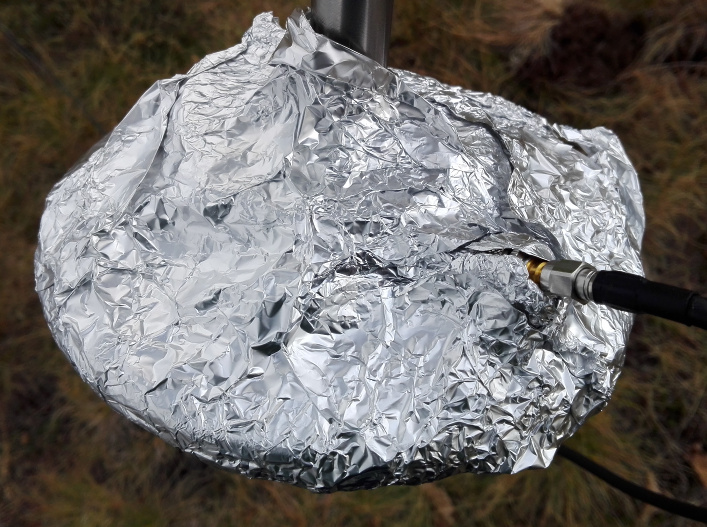
\includegraphics[width=0.40\textwidth]{antenna_foil_cover.jpg}
  \caption[Antenna covered in aluminium foil]
   {Antenna covered in aluminium foil to simulate a jamming attack.}
\end{wrapfigure} 

Step 1 and 2 was designed to trigger the KRL filter, especially the check of solved latitude, longitude and altitude but also the speed, against known values. Step 5 and 6 was also designed to trigger the KRL filter, but more specifically the checking of solved speed. Step 7 and 8 was to designed to reveal what would happen with the both the KRL and the CM filter during a jamming attack as it was believed that covering the antennas with aluminium foil would block all signals out.

\subsection{Observations}\label{observations}
By reviewing the log produced by the Sensor Server, the following was observed:

\begin{itemize}
  \item No false positives, the filters where not triggered before the test started.
  \item The KRL filter was triggered by Sensor 1 at 10:59:19 and cleared at 11:04:35.
  \begin{lstlisting}
    [10/10/16 - 10:59:17] [ ALARM ] Sensor 1 triggered KRL filter!
    ...
    [10/10/16 - 11:04:35] [ ALARM ] Sensor 1 cleared KRL filter!
  \end{lstlisting}
  \item The KRL filter was triggered again at 11:08:27, but this time by Sensor 2. The alarm was cleared at 11:13:43.
    \begin{lstlisting}
    [10/10/16 - 11:08:27] [ ALARM ] Sensor 2 triggered KRL filter!
    ...
    [10/10/16 - 11:13:43] [ ALARM ] Sensor 2 cleared KRL filter!
  \end{lstlisting}
  \item Once again, 11:22:03 the KRL filter was triggered by Sensor 1 and was not cleared until 11:29:21
     \begin{lstlisting}
    [10/10/16 - 11:22:03] [ ALARM ] Sensor 1 triggered KRL filter!
    ...
    [10/10/16 - 11:29:21] [ ALARM ] Sensor 1 cleared KRL filter!
  \end{lstlisting} 
  \item At 11:27.05, it was the CM filter using the clock model that triggered. It stopped triggering 11:27:33. Sensor 2 also triggered the KRL filter 11:27:31 and cleared at 11:34:16.
    \begin{lstlisting}
    [10/10/16 - 11:27:05] [ ALARM ] CSAC Steer value > predicted!
    ...
    [10/10/16 - 11:27:31] [ ALARM ] Sensor 2 triggered KRL filter!
    ...
    [10/10/16 - 11:27:33] [ ALARM ] CSAC Steer value > predicted!
  \end{lstlisting} 
  \item The last 6 seconds, Sensor 2 triggered KRL filter and the CM filter was triggered at multiple occasions.
  \begin{lstlisting}
    [10/10/16 - 11:34:15] [ ALARM ] Sensor 2 triggered KRL filter!
    [10/10/16 - 11:34:16] [ ALARM ] Sensor 2 cleared KRL filter!
    [10/10/16 - 11:34:17] [ ALARM ] Sensor 2 triggered KRL filter!
    [10/10/16 - 11:34:18] [ ALARM ] Sensor 2 triggered KRL filter!
    [10/10/16 - 11:34:19] [ ALARM ] Sensor 2 triggered KRL filter!
    [10/10/16 - 11:34:19] [ ALARM ] CSAC Steer value > predicted!
    [10/10/16 - 11:34:20] [ ALARM ] CSAC Steer value > predicted!
    [10/10/16 - 11:34:20] [ ALARM ] Sensor 2 cleared KRL filter!
    [10/10/16 - 11:34:21] [ ALARM ] CSAC Steer value > predicted!
  \end{lstlisting} 
\end{itemize}

\subsection{Conclusion}
The observations (\ref{observations}) reveals what we expected. After all, when moving a GNSS receivers antenna, the solved position has to change. If it did not, the GNSS receiver or antenna would have to be faulty. Step 5 and 6 (\ref) did not produce the expected result. The altitude, latitude and longitude was expected to be within a safe range, the solved speed on the other hand, was expected to have been way too high. (Kan ha vært pågrunn av at filteret ble lastet med hastighet oppgitt i ms istedet for knop. Dobbeltsjekk dette først.)